\documentclass[11pt]{amsart}
\usepackage[colorlinks=true]{hyperref}
\usepackage{graphicx}
\usepackage{float}
\usepackage{listings}


\title{ScalABM}
\author{David R. Pugh, Daniel F. Tang, J. Doyne Farmer}
\date{\today}

\begin{document}
\maketitle

\section{Objective...}
Our objective is to create a \textit{user-friendly} toolkit for building \textit{scalable}, \textit{data-driven} agent-based models (ABMs) of \textit{economic} systems.

\subsection{Motivation}
Currently the economic ABM community lacks a coherent set of standard tools for testing, developing, and validating their models. The lack of such a toolkit has significantly hindered the progress of agent-based modeling.\footnote{
%
TODO: Compare and contrast our approach with EURACE (and its derivatives), JMAB, Jas-mine, CRISIS, Repast, Swarm, etc.  In particular focus on applications that are economics focused.
%
} 
What we have outlined in the previous section is our vision of what such a ``standard'' should look like. However, in order to avoid...

\begin{figure}[H]
\centering
\includegraphics[width=10cm]{standards.png}
\end{figure}

...we need to maximize the chances that our toolkit gets adopted as a standard. There are a number of facets to our vision that we believe increase the likelihood that our toolkit could be adopted as a standard...
\begin{itemize}
    \item Network effects are key to establishing a standard. We are leveraging recent hardware and software advances (i.e., AWS, Heroku, Scala, Akka, Spark, Cassandra, Neo4j, etc) that are all open-source, free even for commercial-use (specifically Apache 2.0), and that have already generated substantial networks effects in private industry. Users (i.e., undergraduate and graduate students, post-docs, etc) who adopt our toolkit will be learning to tools that will substantially increase the probability of finding a high-paying job (if they choose to leave academia).  Not clear that learning FLAME, Repast, Swarm, Netlogo, Mason, etc would be as useful outside academia. 
    \item Credibility is key to establishing a standard. If you were starting a new scientific ABM project, would you be willing to use software if the source code wasn't available, documentation was sparse, and no unit tests had been written? We are following best practices for software engineering that have been used in previous, successful, open source projects and that have found widespread adoption in private industry. In particular, we will place our source code under version control, develop a rigorous set of unit tests, and strive to maintain a high degree of test and documentation coverage, throughout the lifetime of the project.
\end{itemize}
...additionally...
\begin{itemize}
    \item We should strive to release (early and often!) models from the existing ABM literature as simple example use-cases.    
    \item We should actively seek out partners in private industry for software development expertise.  Many (all?) previous efforts to design toolkits for agent-based modeling have failed due to insufficient attention to software engineering issues. We have been developing networks and contacts in private industry (i.e., Typesafe, Datastax, etc.) that can help us with some of the software engineering challenges. 
    \item We should actively seek out partners in private industry for funding of specific projects that would represent use-cases for our toolkit. The likelihood of finding partners in private industry should be increased by our use of a permissive, open-source license.
\end{itemize}    
\subsection{Requirements}

\subsubsection{User-friendly...}
We expect that users of our ABM toolkit can be classified as either consumers or producers. Consumers are users whose primary objective is to learn about the mechanisms driving a model's key results by playing with model parameters and components. Producers are users whose primary objective is to develop new models using some combination of existing and novel model components.

We want consumers of models built using our framework, particularly those not directly involved with development of any particular model, to be able to easily interact with a model in order to develop intuition and understanding about the mechanisms driving that model's key results.
\begin{itemize}
    \item Models built using our toolkit should have browser-based user interfaces (UIs). Implementing browser-based UIs would allow us to leverage existing, high-quality Javascript libraries for real-time data visualization.
    \item Users should be able to ``play-with'' the model (i.e., tweak model parameters, substitute model components, etc.) from the browser in real-time (i.e., whilst a model is running).
\end{itemize}

We also want to develop a framework that minimizes developer time when either building a new model (or re-configuring an existing model).
\begin{itemize}
    \item Models built using our toolkit should be composed of mostly existing components. This reduces development time for a new model to that needed to create a few novel components together with the time needed to wire all the desired model components together.
    \item The process of wiring model components together, sometimes called dependency injection (DI), should be as simple and transparent as possible.\footnote{
    %
    There are many popular DI approaches (i.e., Guice, Spring, etc). While our framework should not depend on any particular DI library, we should think carefully about what DI library we choose as I expect many users will just mimic our choice.
    %
    }
    \item All model configuration should be done in a \textit{single} file (i.e., some type of application configuration file).  Using this application configuration file it should be possible to reproduce a run of a particular model.
\end{itemize}

\subsubsection{Scalable...}
Aggregate behavior of many (most?) real world social systems fundamentally depends on system size. Therefore in order to accurately model system dynamics we need to be able to run our models as close to observed scale as possible. We need to start thinking about building models ``as if'' we were developing web applications so that we can leverage recent hardware (i.e., massively multi-core servers, cloud computing architectures such as \href{http://aws.amazon.com/}{AWS}, \href{https://www.heroku.com/}{Heroku}, and \href{https://mesosphere.com/}{Mesosphere}, etc) and software advances (specifically \href{http://www.scala-lang.org/}{Scala}, \href{http://akka.io/}{Akka}, etc) that are driving the proliferation of large-scale, distributed web applications in private industry.

\subsubsection{Data-driven...}
We want to build models that can be validated against empirical data and therefore we need to design our toolkit to facilitate this.  Again we should think of our models ``as if'' they are web applications. Web applications consume streams of input data and produce streams of output data; some output data streams are processed and then used again as new input data streams. With all of this data flowing around, database integration and data processing are crucial components of web application \textit{design}. We should design our toolkit to integrate cleanly with database architectures, such as \href{http://cassandra.apache.org/}{Apache Cassandra} and \href{http://neo4j.com/}{Neo4j}, and data processing engines, such as \href{http://spark.apache.org/}{Apache Spark}, that are specifically designed to support large-scale web applications.

\subsubsection{Economic...}
Finally, we are not seeking to build a general purpose toolkit for agent-based modeling. Rather we want to build a toolkit that is designed to facilitate the construction of agent-based models of economic systems.

An economy is populated with many seemingly disparate types of agents (i.e., consumers, producers, financiers, government, some markets, etc). We need to distill the core essence (in terms of data and behaviors) of these different agents into a multi-layered Application Programming Interface (API) defining a generic \textit{economic agent} that can then be specialized to the various types of economic agents needed for any particular model. Our hope is that by doing this we can reduce the effort needed for the parts of agent-based modeling that consume a great deal of software development time, such as accounting or contract enforcement.  We also hope that by identifying the key components we can build standard, highly modular interfaces that make it easy to interchange components of models.

\subsubsection{Reproducible...}
Results of many (most?) ABMs are not easily reproducible. More often then not, source code for models used in published articles is not publicly available. Reproducibility is further hindered by the lack of use of ``best practices'' for software development (in particular unit testing). Documentation is typically lacking. 

In order to address these issues and make models built using our toolkit reproducible we should develop the toolkit \textit{from the beginning} as an open-source project and should exemplify ``best practices'' in software engineering: version control using \href{https://git-scm.com/}{Git} and \href{https://github.com/}{GitHub}; continuous integration of unit tests using \href{https://travis-ci.org/}{Travis CI} or \href{https://jenkins-ci.org/}{Jenkins}; static analysis of source code using \href{https://www.codacy.com/login}{Codacy}, \href{https://codeclimate.com/}{Code Climate}, etc; documentation should be extensive, written along with the code, and publicly hosted on GitHub.   

\subsection{Coarse-grain architecture}
We want to mimic the layered architecture of a modern distributed web application.  The coarse-grained archictecure of ScalABM consists of five layers.
\begin{itemize}
    \item Cluster Management Layer: Base layer for the entire framework. We will not need to build this layer. We can simply use third-party cluster management tools. Mesos, Amazon EC2, Hadoop/Yarn.  Probably best to package our application up in a ``container'' of some kind (i.e., Docker, etc) and then ship it to a third party cloud computing service that manages a cluster and who can then scale up our application.  Note that, unlike EURACE, we will NOT need to have access to a university or governmental super computer to scale up our application.
    \item User Interface Layer:
    \item Data Analytics Layer:
    \item Model Layer:
    \item Database Layer:
\end{itemize}

\begin{figure}[H]
\centering
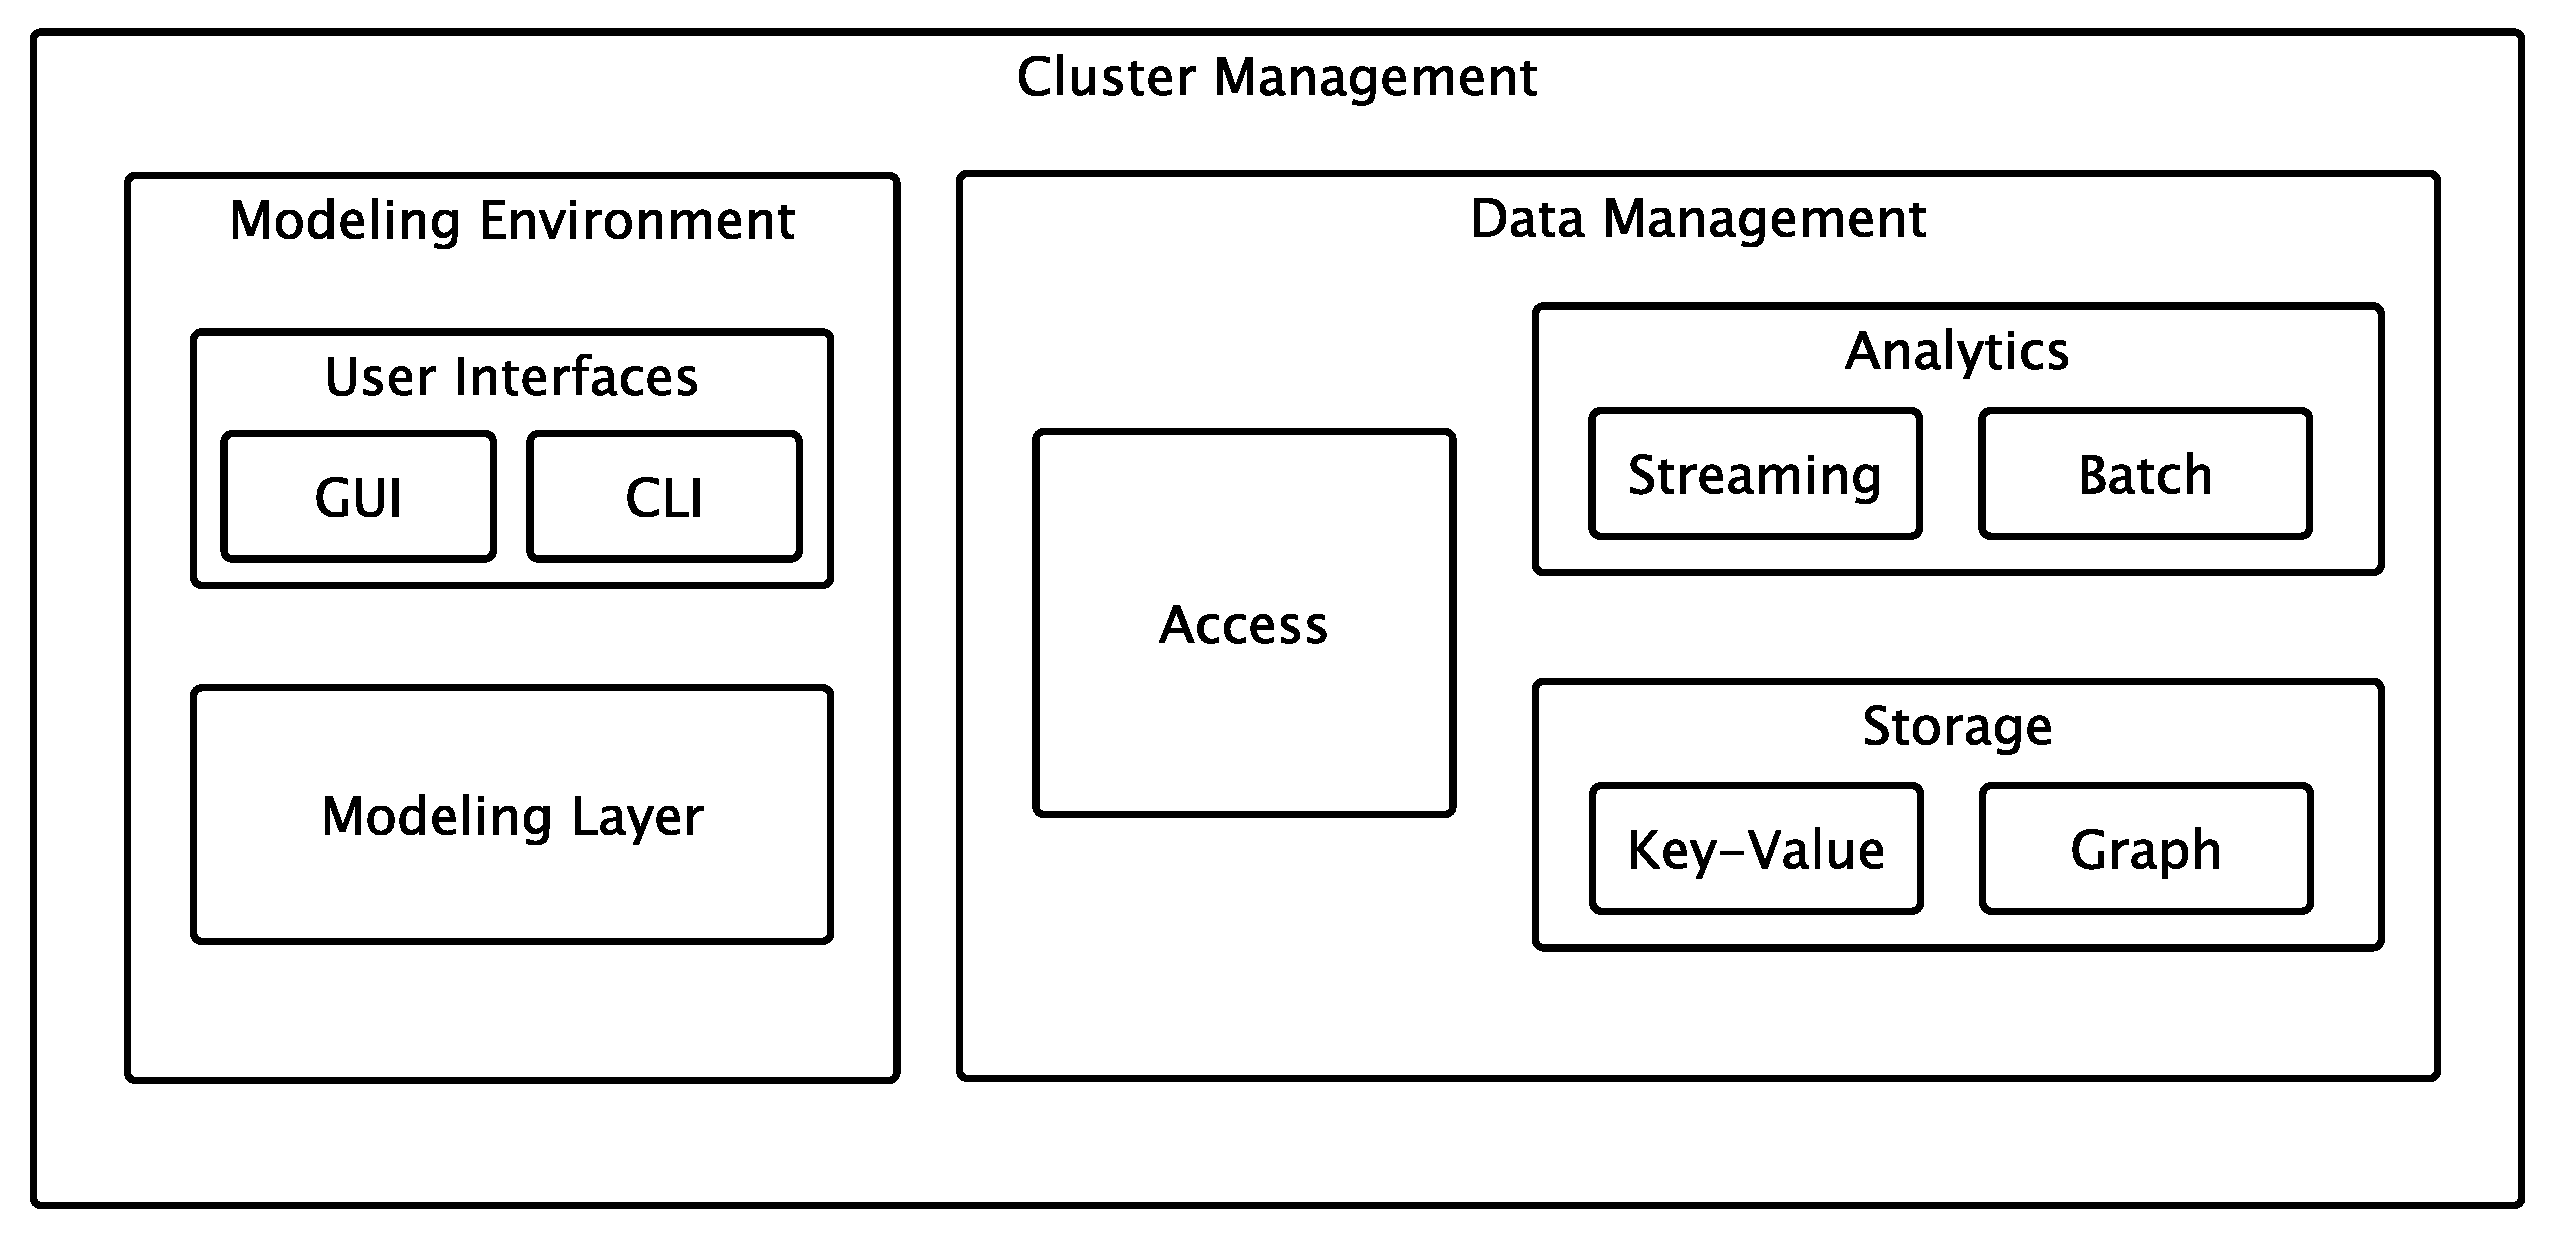
\includegraphics[width=10cm]{coarse-grain-schema.pdf}
\caption{Coarse-grain architecture for ScalABM. }
\end{figure}



% \section{Economics as distributed computation}
% Major source of motivation for our approach is Rob Axtell's \href{http://www.researchgate.net/profile/Robert_Axtell2/publication/228586815_Economics_as_distributed_computation/links/0a85e536b81c27f06e000000.pdf}{2002 Brookings working paper}.

% \subsection{Concurrency vs parallelism}
% Discuss the difference between parallelism and concurrency. See this \href{http://stackoverflow.com/questions/1050222/concurrency-vs-parallelism-what-is-the-difference}{SO} post for details. Concurrency is a more general type of parallelism. Economic systems are concurrent.

% \subsection{Asynchronous vs synchronous}
% Discuss the difference between synchronous and asynchronous execution. Economic systems are asynchronous not synchronous.

% \subsection{Economics is concurrent, asynchronous distributed computing}
% Concurrent, asynchronous In his , Rob discusses have noted that the economy is a distributed system which provides a motivation for our use of Scala and Akka to implement our framework (both were developed specifically for building scalable distributed systems). Contrast with other ABM frameworks, programming lanaguages, etc.

%There is a sense in which economics can be reduced to a combination of accounting and agent decision making.  

\end{document}
